\documentclass[border=10pt]{standalone}
\usepackage{tikz}
\usetikzlibrary{arrows.meta, shapes, positioning, fit, calc, backgrounds}

\begin{document}
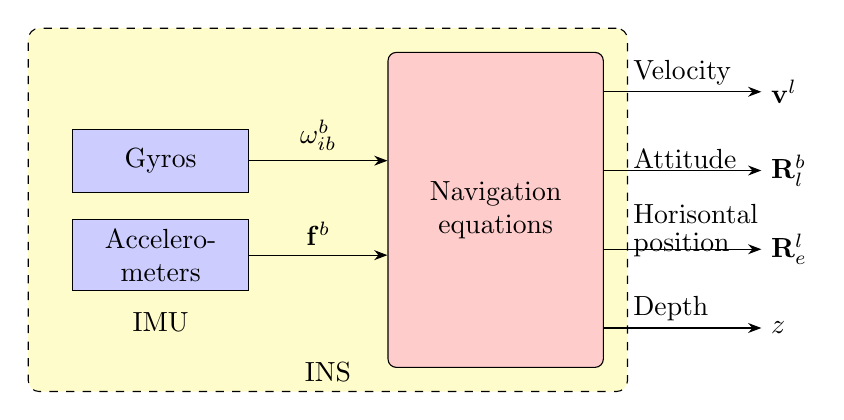
\begin{tikzpicture}[
    block/.style={rectangle, draw, fill=blue!20, text width=2cm, align=center, minimum height=0.8cm},
    navblock/.style={rectangle, draw, rounded corners=3pt, fill=red!20, text width=2.5cm, align=center, minimum height=4cm},
    container/.style={rectangle, draw, dashed, rounded corners=4pt, fill=yellow!20},
    imucontainer/.style={rectangle, draw, dashed, rounded corners=4pt, fill=blue!10},
    arrow/.style={->, >=Stealth, thin}
]

% IMU blocks
\node[block] (gyros) at (0,1) {Gyros};
\node[block] (accel) at (0,-0.2) {Accelero-\\meters};

% IMU container
\begin{scope}[on background layer]
\node[imucontainer, fit=(gyros)(accel), inner xsep=0.25cm, inner ysep=0.7cm] (imu) {};
\end{scope}
\node at ($(imu.south)+(0,0.32cm)$) {IMU};

% Navigation equations block
\node[navblock, right=1.5cm of imu] (nav) {Navigation\\equations};

% INS container
\begin{scope}[on background layer]
\node[container, fit=(imu)(nav), inner sep=0.3cm] (ins) {};
\end{scope}
\node at ($(ins.south)+(0,0.25cm)$) {INS};

% Arrows from IMU to Navigation
\draw[arrow] (gyros.east) -- node[above] {$\omega^b_{ib}$} (nav.west |- gyros.east);
\draw[arrow] (accel.east) -- node[above] {$\mathbf{f}^b$} (nav.west |- accel.east);

% Output arrows and labels
\draw[arrow] (nav.east) ++(0, 1.5) -- ++(2,0) node[right] {$\mathbf{v}^l$};
\draw[arrow] (nav.east) ++(0, 0.5) -- ++(2,0) node[right] {$\mathbf{R}_l^b$};
\draw[arrow] (nav.east) ++(0, -0.5) -- ++(2,0) node[right] {$\mathbf{R}_e^l$};
\draw[arrow] (nav.east) ++(0, -1.5) -- ++(2,0) node[right] {$z$};

% Labels on the navigation outputs
\node[anchor=west] at ($(nav.east)+(0.25cm,1.75cm)$) {Velocity};
\node[anchor=west] at ($(nav.east)+(0.25cm,0.65cm)$) {Attitude};
\node[anchor=west] at ($(nav.east)+(0.25cm,-0.05cm)$) {Horisontal};
\node[anchor=west] at ($(nav.east)+(0.25cm,-0.45cm)$) {position};
\node[anchor=west] at ($(nav.east)+(0.25cm,-1.25cm)$) {Depth};

\end{tikzpicture}
\end{document}
